% !TEX root = ../om_ts_04.tex

\begin{frame} % название фрагмента

\videotitle{MA процессы}

\end{frame}



\begin{frame}{MA процессы: план}
  \begin{itemize}[<+->]
    \item Определение и запись с лагами. 
    \item Стационарность. 
    \item ACF и PACF.
    \item Неединственность записи. 
  \end{itemize}

\end{frame}

\begin{frame}
  \frametitle{Лаговый оператор}

  \begin{block}{Определение}
    Для процесса $(y_t)$, определённого при $t \in \mathbb{Z}$, \alert{лагированным} процессом 
    $L y_t$ называют ту же последовательность величин со сдвинутым индексом,
    \[
      L y_t = y_{t-1}.
    \]
  \end{block}

  \pause
  \[
  L^2 y_t = L\cdot L\cdot y_t = L\cdot y_{t-1} = y_{t-2}.  
  \]
  \pause
  \[
  \Delta y_t = y_t - y_{t-1} = (1 - L) y_t.  
  \]
  \pause
  \[
  \Delta_{12} y_t = y_t - y_{t-12} = (1 - L^{12}) y_t.  
  \]
\end{frame}

\begin{frame}
  \frametitle{MA процесс}

  \begin{block}{Определение}
    Процесс $(y_t)$, который \alert{можно} представить в виде
    \[
    y_t = \mu + u_t + \alpha_1 u_{t-1} + \ldots + \alpha_q u_{t-q},  
    \]
    где $\alpha_q \neq 0$ и $(u_t)$ — белый шум, называют $MA(q)$ процессом. 
    
    \alert{MA — Moving Average — скользящее среднее}. 
  \end{block}
  
  \pause
  Пример $MA(1)$ процесса:
  \[
    y_t = 5 + u_t + 0.3 u_{t-1},
  \]
  где $(u_t)$ — некоторый белый шум.
  \pause

  Нормировка коэффициента при $u_t$ \alert{к единице}.

\end{frame}

\begin{frame}
  \frametitle{Запись с лагами}

  \begin{block}{MA с лаговым полиномом}
    Процесс $(y_t)$, который \alert{можно} представить в виде 
    \[
    y_t = \mu + P(L) u_t,  
    \]
    где $P(L)$ — многочлен степени $q$ от лага $L$ с $P(0)=1$, а $(u_t)$ — белый шум,
    называют $MA(q)$ процессом. 
  \end{block}

  \pause
  Пример $MA(2)$ процесса:
  \[
  y_t = 5 + (1 - 0.2 L + 0.3 L^2) u_t,
\]
где $(u_t)$ — белый шум. 
\end{frame}


\begin{frame}
  \frametitle{Стационарность MA}

  \begin{block}{Теорема}
    Любой $MA(q)$ процесс стационарен. 
  \end{block}

  \pause
  \begin{block}{Доказательство на примере}
    \[
      \E(5 + u_t + 0.6u_{t-1} + 0.2u_{t-2}) = 5
    \]
    \pause
    \begin{multline*}
      \Cov(5 + u_t + 0.6u_{t-1} + 0.2u_{t-2}, \\
      5 + u_{t+k} + 0.6u_{t+k-1} + 0.2u_{t+k-2}) = \gamma_k
    \end{multline*}
    Ковариация для $(u_t)$ определяется \alert{совпадающими} индексами. 

    При изменении $t$ совпадающие индексами пары те же.
  \end{block}
  

\end{frame}

\begin{frame}
  \frametitle{ACF}

  \begin{block}{Теорема}
    У $MA(q)$ процесса теоретическая автокорреляция $\rho_k$ равна нулю при $k>q$
  \end{block}
  \pause
  \begin{block}{Доказательство}
    Считаем $\gamma_3 = \Cov(y_t, y_{t+3})$ для $MA(2)$:
    \[
    \gamma_3 = \Cov(5 + u_t + 0.6u_{t-1} + 0.2u_{t-2}, 5 + u_{t+3} + 0.6u_{t+3-1} + 0.2u_{t+3-2}) = 0
    \]
    \alert{Нет совпадающих} индексов у белого шума!
  \end{block}
  \pause 
  Побочный результат: для $MA(q)$ процесса $\rho_q \neq 0$.
\end{frame}


\begin{frame}
  \frametitle{PACF}

  \begin{block}{Теорема}
    У $MA(q)$ процесса теоретическая частная автокорреляция $\varphi_{kk}$ \alert{экспоненциально} быстро 
    сходится к нулю.
  \end{block}
  \pause
  \[
  \abs{\varphi_{kk}} < b_0 \cdot r^k, \text{ где } r \in (0;1).
  \]

  

\end{frame}

\begin{frame}
  \frametitle{ACF и прогнозы}

  Традиционно $MA(q)$ процесс оценивают предполагая совместную нормальность $(y_t)$. 

  \pause
  Из нулевой $\rho_k=0$ при $k>q$ следует независимость $y_t$ и $y_{t+k}$.
  
  \pause
  Прогнозы больше, чем на $q$ шагов вперёд, совершенно одинаковые. 

  \[
      (y_{T+q + 1} \mid \mathcal{F}_T) \sim (y_{T+q + 2} \mid \mathcal{F}_T) \sim (y_{T+q + 3} \mid \mathcal{F}_T) \sim \ldots 
  \]
\end{frame}

\begin{frame}
  \frametitle{Прогнозы для $MA(2)$}

  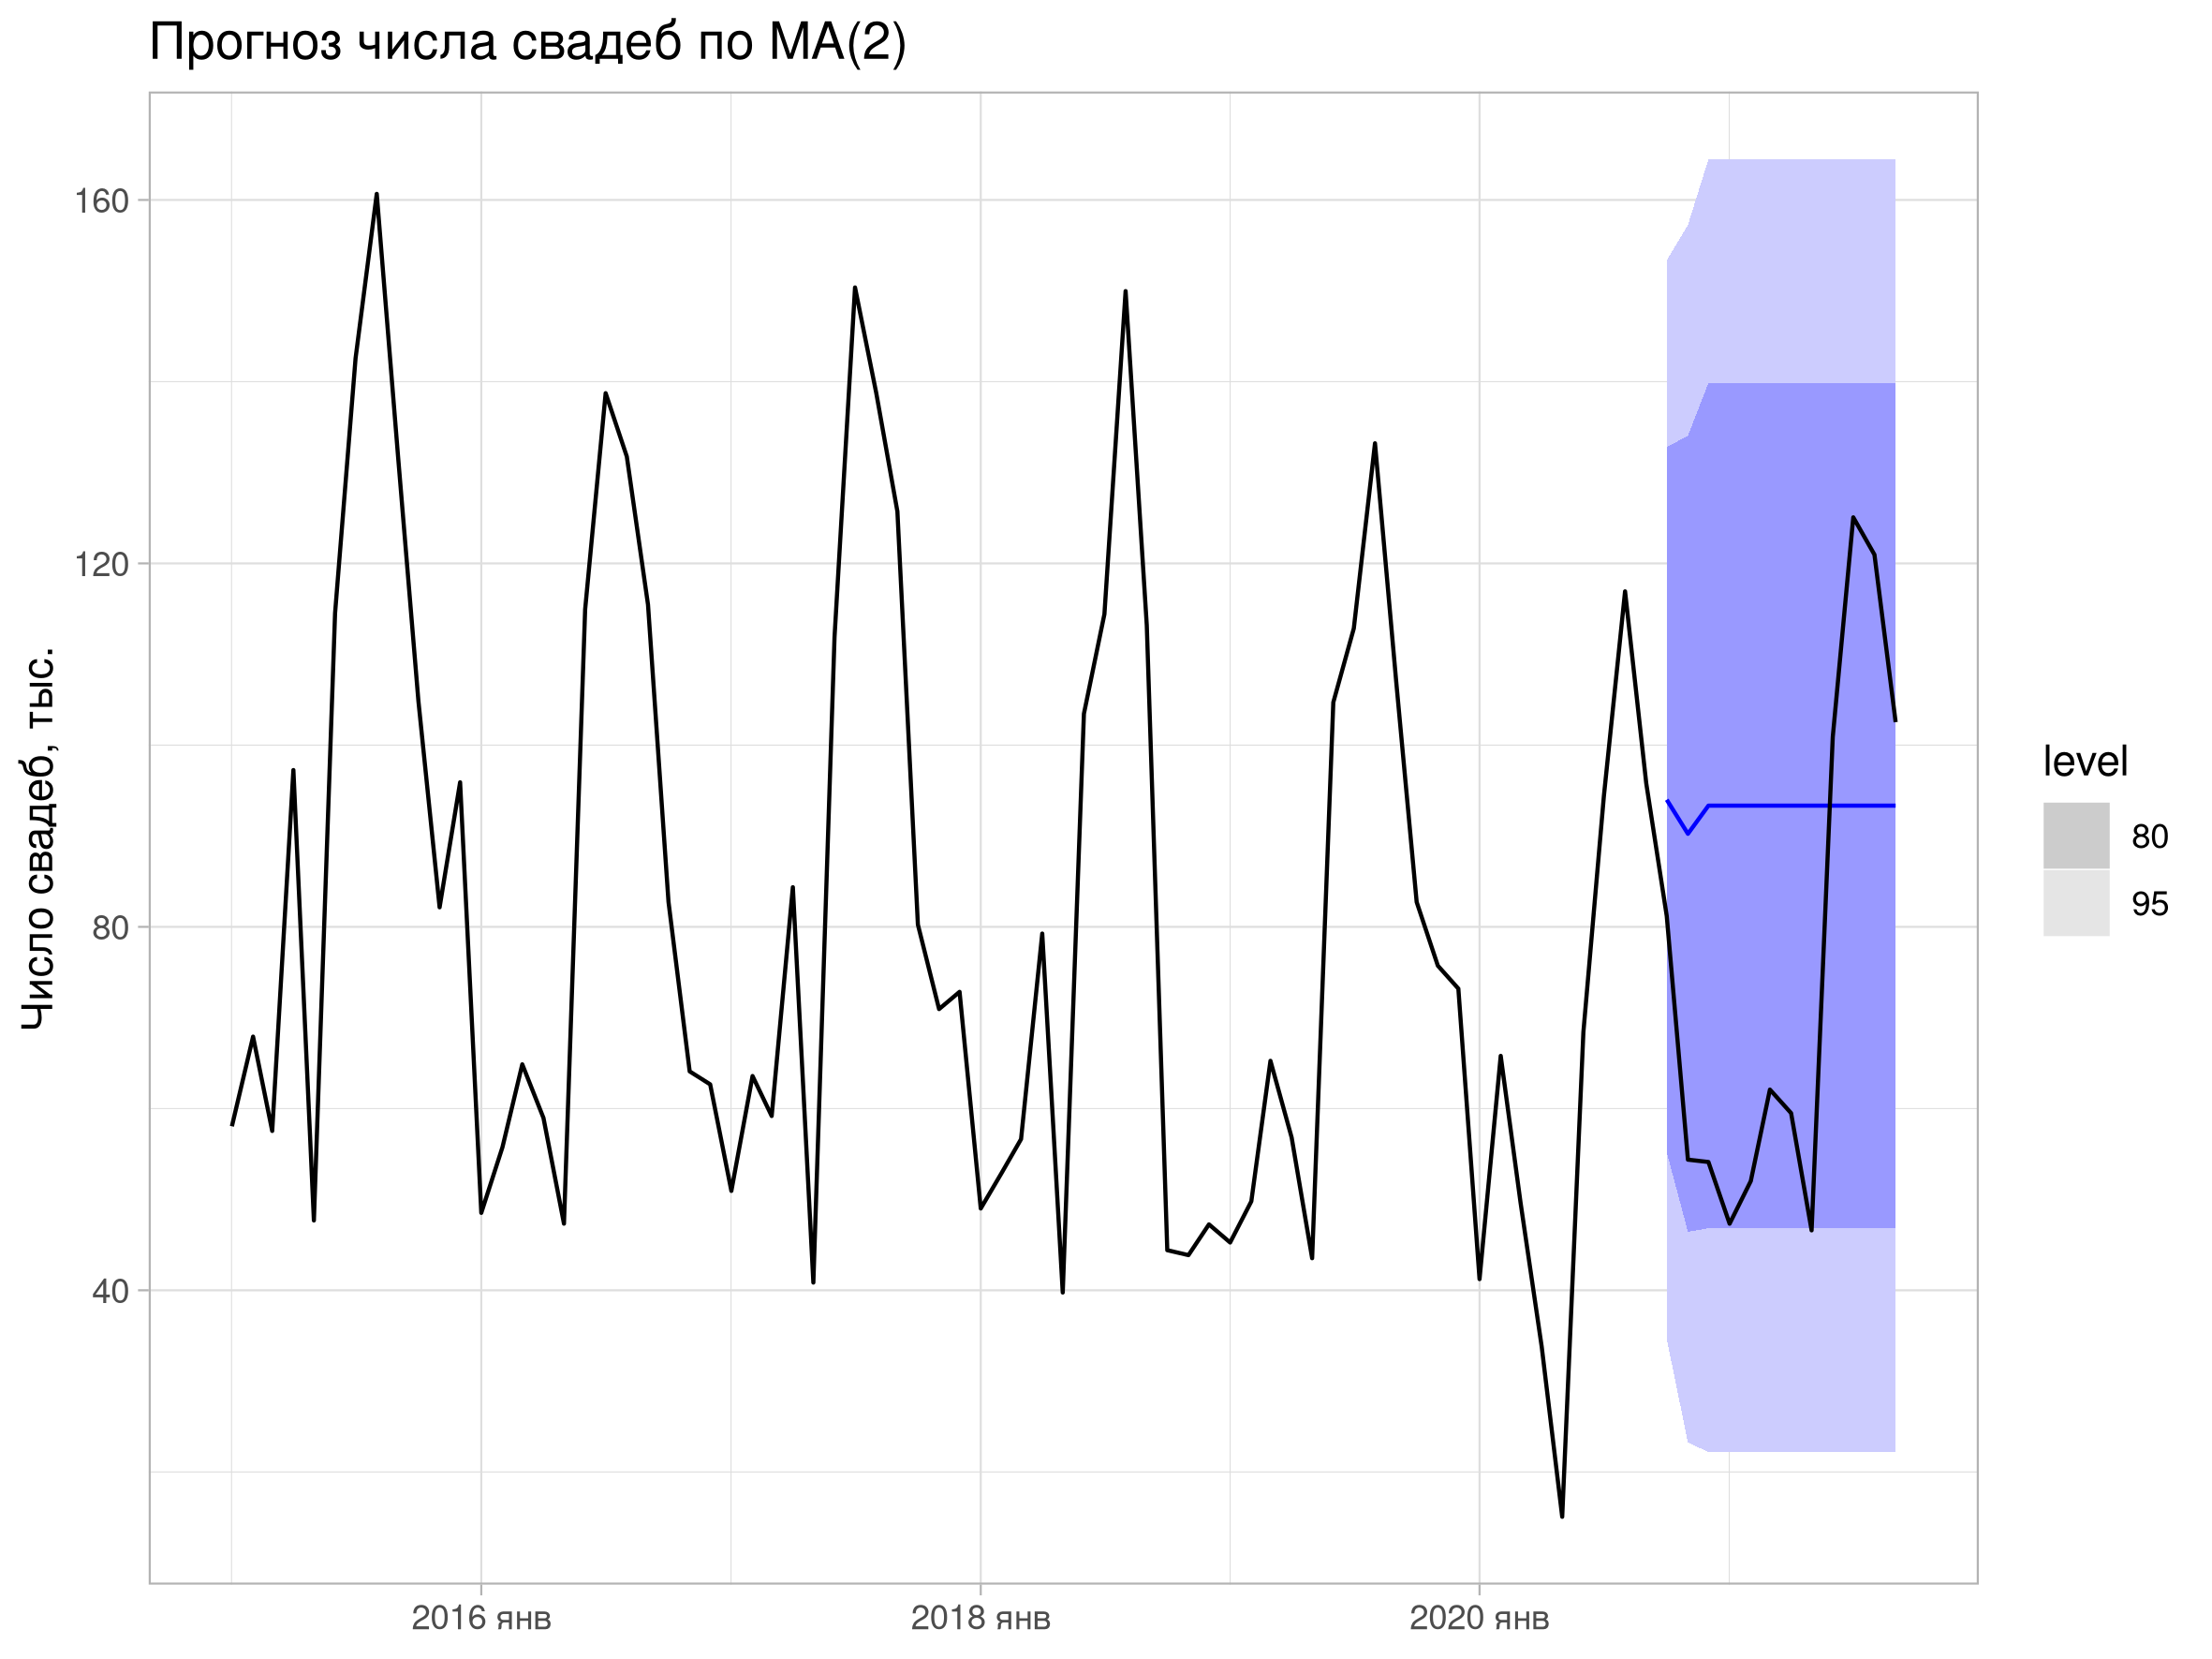
\includegraphics[width=\textwidth]{pictures/om_ts_04-094.png}
  

\end{frame}


\begin{frame}
  \frametitle{А корректно ли определение?}
  
  Нюанс: $(y_t)$ — наблюдаемый ряд, $(u_t)$ — \alert{единорог}.

  \pause

  Машенька: этот $y_t$ — $MA(1)$ процесс.

  Вовочка: этот $y_t$ — $MA(2)$ процесс. 

  \pause 

  Так \alert{не бывает!}

\end{frame}



\begin{frame}
  \frametitle{Однако!}

  Машенька: этот $y_t$ — $MA(1)$ процесс с уравнением

  \[
    y_t = 5 + u_t + 0.5 u_{t-1}, \quad \sigma^2_u = 4.
  \]

  Вовочка: этот $y_t$ — $MA(1)$ процесс с уравнением

  \[
    y_t = 5 + u_t + 2 u_{t-1}, \quad \sigma^2_u = 1.
  \]

  \pause
  Здесь \alert{нет противоречия}: $(u_t)$ — единорог!
\end{frame}

\begin{frame}
  \frametitle{Противоречия нет}

  Машенька: этот $y_t$ — $MA(1)$ процесс с уравнением

  \[
    y_t = 5 + \nu_t + 0.5 \nu_{t-1}, \quad \sigma^2_{\nu} = 4.
  \]

  Вовочка: этот $y_t$ — $MA(1)$ процесс с уравнением

  \[
    y_t = 5 + u_t + 2 u_{t-1}, \quad \sigma^2_u = 1.
  \]
  \pause
  Связь $(u_t)$ и $(\nu_t)$:
  \[
  (1+0.5L)\nu_t = (1+2L)u_t.  
  \]
\end{frame}



\begin{frame}{MA процессы: итоги}

  \begin{itemize}[<+->]
    \item $MA(q)$ — взвешивание нескольких белых шумов. 
    \item $MA(q)$ — стационарный процесс. 
    \item $ACF$ резко зануляется, $PACF$ стремится к нулю.
    \item Неединственность записи. 
  \end{itemize}
\end{frame}



